\section{Aufbau von M$^2$etis}
\label{chap:aufbau_metis}
Dieses Kapitel erläutert den Aufbau von \ac{m2etis} und zeigt den Rahmen sowie die Einordnung der Publish/Subscribe-Komponente in das Framework. Wie eingangs erwähnt, zielt das Framework auf eine optimale Verteilung \emph{aller} Eventtypen im \ac{mmve}. Dabei wird nicht der klassische Ansatz einer Client-Server-Kommunikation, sondern ein dezentraler Ansatz mit einem Publish/Subscribe-System auf einem \ac{p2p}-Netzwerk, gewählt \cite{Fischer2010a}.

\Fref{fig:metis_aufbau} zeigt die zeitliche Aufteilung des Systems in \emph{Konzeption} und \emph{Laufzeit} sowie die Schnittpunkte von \ac{m2etis} mit dem \ac{mmve}. In der Grafik wird dieses durch ein \emph{Spiel} dargestellt. \emph{Konzeption} beschreibt hier die gesamten Tätigkeiten vor der Nutzung von \ac{m2etis} durch das \ac{mmve}. Im ersten Schritt werden die genutzten Eventtypen durch den Entwickler des \acp{mmve} identifiziert und anhand der vorgegebenen Dimensionen semantisch beschrieben. Im zweiten Schritt verarbeitet der \ac{m2etis} \emph{Optimierer} diese Beschreibungen unter Zuhilfenahme des \emph{semantischen Modells} und des \emph{Kostenmodells}. Dieser Schritt nutzt zur Erzeugung der optimierten \emph{Kanäle} die verschiedenen konkreten Implementierungen der sieben Dimensionen. \ac{m2etis} wird -- nach Fertigstellung -- eine Auswahl an Implementierungen mitliefern, ist jedoch offen für vom Nutzer geschriebene Implementierungen.
Die optimierten Kanäle lassen sich zur Laufzeit (im 3. Schritt) über die Publish/Subscribe-API ansprechen und kommunizieren über das \ac{p2p}-Netzwerk. Ein Kanal bündelt dabei die verschiedenen Implementierungen und zieht diese zur Bearbeitung der Events heran. Um die Benutzung der Frameworks zu vereinfachen, soll die Kanaloptimierung transparent erfolgen und das \ac{mmve} zur Laufzeit keine Implementierungsdetails der Kanäle kennen, sondern diese rein über die generische API ansprechen.


\begin{figure}[htbp]
\centering
\resizebox{\textwidth}{!}{%
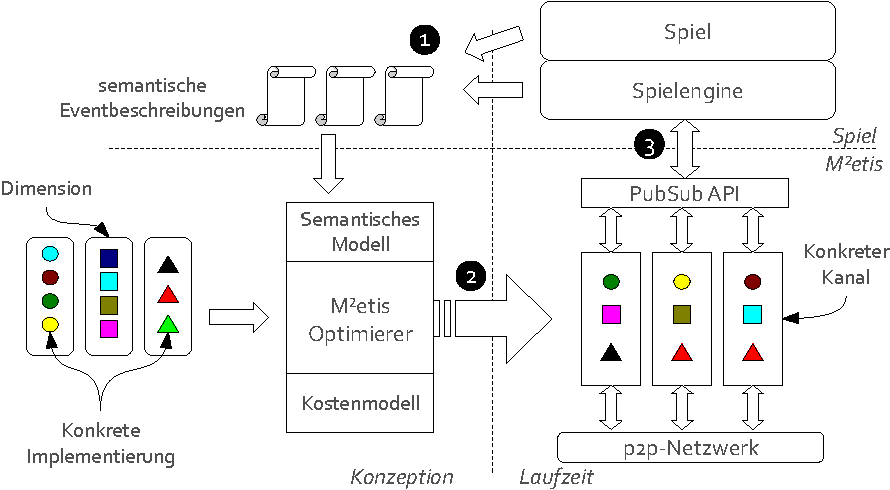
\includegraphics{grafics/metis_aufbau.pdf}}
\caption{Architekturübersicht von M$^2$etis}
\label{fig:metis_aufbau}
\end{figure}


Diese Arbeit beschränkt sich auf die Anbindung des gewählten \ac{p2p}-Netzwerk und die Konzeption des Publish/Subscribe-Systems. Damit das Framework frühzeitig einsetzbar ist und weitere Arbeiten darauf aufbauen können, wird zudem eine prototypische Implementierung des Publish/Subscribe-Systems erstellt. Die Konzeption der semantische Beschreibung von Eventtypen, die Konzeption des Kostenmodells und die Entwicklung des Optimierers würden den Rahmen dieser Diplomarbeit sprengen und bleiben nachfolgenden Arbeiten überlassen.
